\chapter{Ergebnisse}

Wenn wir unsere Programm auführen erhalten wir folgende Ausgabe:

\begin{figure}[h]
    \begin{center}
        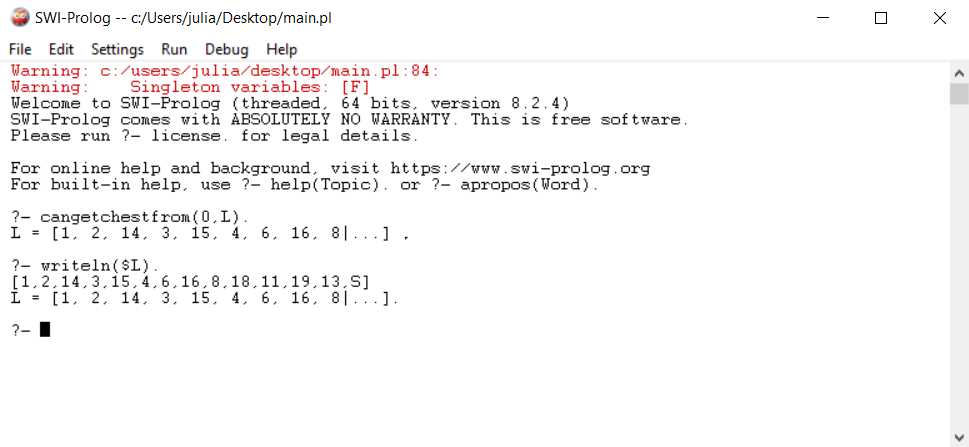
\includegraphics[width=1\textwidth]{content/pictures/output.png}
        \caption{Output Prolog Keys and Doors}
        \label{fig:output}
    \end{center}
\end{figure}

\noindent
Wie auf der Abbildung zu erkennen ist, braucht der Agent genau 13 Schritte bis
er beim Schatz angekommen ist. Dies ist nur eine von mehreren Lösungen, welche 
das Programm haben könnte.